\documentclass[margin,line]{res}
\usepackage{graphicx}
\usepackage{verbatim}
\usepackage{url}
\urlstyle{same}

\usepackage[utf8]{inputenc}
\usepackage[T1]{fontenc}

\oddsidemargin -.5in
\evensidemargin -.5in
\textwidth=6.0in
\itemsep=0in
\parsep=0in

\newenvironment{list1}{
  \begin{list}{\ding{113}}{%
      \setlength{\itemsep}{0in}
      \setlength{\parsep}{0in} \setlength{\parskip}{0in}
      \setlength{\topsep}{0in} \setlength{\partopsep}{0in} 
      \setlength{\leftmargin}{0.17in}}}{\end{list}}
\newenvironment{list2}{
  \begin{list}{$\bullet$}{%
      \setlength{\itemsep}{0in}
      \setlength{\parsep}{0in} \setlength{\parskip}{0in}
      \setlength{\topsep}{0in} \setlength{\partopsep}{0in} 
      \setlength{\leftmargin}{0.2in}}}{\end{list}}

\begin{document}

\name{
\begin{tabular*}{7.4in} {@{\extracolsep{\fill}}lr}
Toby Dylan Hocking & Curriculum Vitae 
\end{tabular*}
}

\begin{resume}
\section{\sc Contact and General Info}
\vspace{.05in}
\begin{tabular*}{6.1in} {@{\extracolsep{\fill}}ll}
  {\bf Northern Arizona University}& Birth: 17 March 1984 in Newport Beach, California\\
  Tenure-Track Assistant Professor  & Citizenship: USA \\
   2018-present
 & Languages: English (native), French (fluent).\\
  Web: \url{http://tdhock.github.io} &   E-mail:  toby.hocking@nau.edu \\
\end{tabular*}

\section{\sc Research Interests}

Fast, accurate, and interpretable machine learning algorithms, with
applications in cybersecurity, genomics, neuroscience, medicine,
microbiome, robotics, satellite/sonar imagery,
climate modeling.


\section{\sc Honors and Awards (Selected) \\ \hspace{0.1cm} \\ 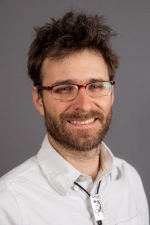
\includegraphics[width=3cm]{HOCKING-rectangle-lores.jpg}}

PI on travel grant from DATAIA (Artificial Intelligence Institute of
Université Paris-Saclay), 24,000 euros, Academic year
2024--2025. ``Efficient algorithms and software for change-point
detection.''

PI on National Science Foundation grant 2303612, US\$731,881, Sep
2023--Aug 2025. ``POSE: Phase II: Expanding the data.table ecosystem
for efficient big data manipulation in R.''

Co-PI on National Institutes of Health grant, US\$455,660, Aug 2023 to
July 2027. ``Addressing Structural Determinants of Autism Disparities
via Cross-Sector Analysis of Secondary Data.'' US\$200K under my control =
US\$50K in each of 4 academic years.

Co-PI on National Science Foundation grant, US\$3,600,000, Sept 2022 to
Sept 2025. ``Friends and Foes: microbial interactions and soil
biogeochemistry after 23 years of experimental warming.'' 
US\$30K under my control = US\$10K in each of 3 academic years.

Co-PI on National Science Foundation grant, US\$2,300,000, Sept 2021
to Aug 2026. ``MIM: Discovering in reverse – using isotopic
translation of omics to reveal ecological interactions in
microbiomes.''  US\$200K under my control = US\$40K in
each of 5 academic years.

Air Force Research Laboratory, Summer Faculty Fellowship, US\$20,000,
May--July 2021, ``Machine learning algorithms for understanding
physically unclonable functions based on resistive memory devices.''

PI on R Consortium Grant, US\$34,000, Jan--Dec 2020, ``RcppDeepState: an easy
way to fuzz test compiled code in R packages.''

\section{\sc Peer-reviewed publications (Selected)}

Hillman J, {\bf Hocking TD}. Optimizing ROC Curves with a Sort-Based
Surrogate Loss Function for Binary Classification and Changepoint
Detection. {\it J. Machine Learning Research} 24(70):1-24, 2023.

{\bf Hocking TD}, Barr J, Thatcher T. Interpretable linear models for predicting security vulnerabilities in source code. 2022 Fourth International Conference on Transdisciplinary AI (TransAI). 

Drouin A, {\bf Hocking TD}, Laviolette F. Maximum margin interval
trees. {\it Neural Information Processing Systems (NeurIPS)}, 2017.

{\bf Hocking TD}, Rigaill G, Bourque G. PeakSeg: constrained optimal
segmentation and supervised penalty learning for peak detection in
count data. {\it International Conference on Machine Learning (ICML)},
2015.

{\bf Hocking TD}, Rigaill G, Bach F, Vert J-P. Learning sparse
penalties for change-point detection using max-margin interval
regression. {\it International Conference on Machine Learning (ICML)}, 2013.

{\bf Hocking TD}, Joulin A, Bach F, Vert J-P. Clusterpath: an
Algorithm for Clustering using Convex Fusion Penalties. {\it International Conference on Machine Learning (ICML)}, 2011.


\end{resume}
\end{document}




